% last updated in April 2002 by Antje Endemann
% Based on CVPR 07 and LNCS, with modifications by DAF, AZ and elle, 2008 and AA, 2010, and CC, 2011; TT, 2014

\documentclass[runningheads]{llncs}
\usepackage[width=122mm,left=12mm,paperwidth=146mm,height=193mm,top=12mm,paperheight=217mm]{geometry}

\usepackage{graphicx}

\usepackage{amsmath,amssymb} % define this before the line numbering.
\usepackage{ruler}
\usepackage{color}
% \usepackage{subfigure}
% 
% \usepackage{setspace}
\usepackage{algorithm}
\usepackage{epsfig}
% \usepackage[noend]{algorithmic}
% \newtheorem{thm}{Theorem}
\graphicspath{{./Figure/}} 
\definecolor{orange}{rgb}{1,0.5,0}
\definecolor{darkgreen}{rgb}{0,0.5,0}
\definecolor{darkblue}{rgb}{0,0,0.5}

\def\etal{et al.\ }
\def\ie{i.e.\ }
\def\eg{e.g.\ }

%put a wide hat over the argumetn
\newcommand{\lift}[1]{\ensuremath{\widehat{#1}}}

%put a wide hat over the argumetn
%\newcommand{\lifto}[1]{\ensuremath{\check{#1}}}
\newcommand{\lifto}[1]{\ensuremath{\overset{_{_{\circ}}}{#1}}}


% stack vector
\newcommand{\stackv}[1]{\ensuremath{\vet{v}\left( {#1} \right)}}
\newcommand{\ustackv}[1]{\ensuremath{\inv{\vet{v}}\left( {#1} \right)}}

% symmetric stack vector
\newcommand{\stackvs}[1]{\ensuremath{\vet{v}_{\textit{sym}}\left( {#1} \right)}}

% Matrix Lifting: put a wide hat over the argument intended to be a matrix
\newcommand{\mlift}[1]{\ensuremath{\lift{\mat{#1}}}}
\newcommand{\mlifto}[1]{\ensuremath{\lifto{\mat{#1}}}}

% Vector Lifting: put a wide hat over the argument intended to be a matrix
\newcommand{\vlift}[1]{\ensuremath{\lift{\vet{#1}}}}
\newcommand{\vlifto}[1]{\ensuremath{\lifto{\vet{#1}}}}

\newcommand{\bmat}[1]{\ensuremath{\begin{bmatrix} #1 \end{bmatrix}}}
% Vector: print the argument as a vector
\newcommand{\vet}[1]{\ensuremath{\mathbf{#1}}}

% Matrix: print the argument as a matrix
\newcommand{\mat}[1]{\ensuremath{\,\mathtt{#1}\,}}

% Inverse: print a -1 on the top right of the argument 
\newcommand{\inv}[1]{\ensuremath{{#1}^{\text{-}1}}}

% Inverse: print a -1 on the top right of the argument 
\newcommand{\minv}[1]{\ensuremath{\mat{{#1}}^{\text{-}1}}}

% Transpose: print a T on the top right of the argument 
\newcommand{\tra}[1]{\ensuremath{{#1}^{\!\mathsf{T}}}}

% Transpose Matrix: print a T on the top right of the argument intended to be a matrix 
\newcommand{\mtra}[1]{\ensuremath{\tra{\mat{#1}}}}

% Transpose Vector: print a T on the top right of the argument intended to be a vector
\newcommand{\vtra}[1]{\ensuremath{\tra{\vet{#1}}}}

% minus transpose:  print a -T on the top right of the argument
\newcommand{\ment}[1]{\ensuremath{{#1}^{\text{-}\mathsf{T}}}}

% minus transpose matrix:  print a -T on the top right of the argument
\newcommand{\mment}[1]{\ensuremath{{\mat{#1}}^{\text{-}\mathsf{T}}}}

% Cross Matrix:  print the argument in the cross matrix notation
\newcommand{\crmat}[1]{\ensuremath{\left[{#1}\right]_{\times}}}

\newcommand{\mattwoone}[2]{\ensuremath{\left( \begin{array}{c} #1 \\ #2 \\ \end{array} \right)}}

\newcommand{\mattwotwo}[4]{\ensuremath{\left( \! \begin{array}{cc} #1 & #2 \\ #3 & #4 \\ \end{array} \! \right)}}

\newcommand{\matthreethree}[9]{\ensuremath{\left( \begin{array}{ccc} #1 & #2 & #3 \\ #4 & #5 & #6 \\ #7 & #8 & #9 \\ \end{array} \right)}}

\newcommand{\Vi}{\ensuremath{\mat{V}_{\!i}}}
\newcommand{\VF}{\ensuremath{\mat{V}^{\!F}}}
\newcommand{\VB}{\ensuremath{\mat{V}^{\!B}}}
\newcommand{\VirtualF}[1]{\ensuremath{\hat{\mat{#1}}^{\!F}}}
\newcommand{\VirtualB}[1]{\ensuremath{\hat{\mat{#1}}^{\!B}}}
\newcommand{\VFi}{\ensuremath{\mat{V}^{\!F}_{\!i}}}
\newcommand{\VBi}{\ensuremath{\mat{V}^{\!B}_{\!i}}}
\newcommand{\VirtualFi}[1]{\ensuremath{\hat{\mat{#1}}^{\!F}_{\!i}}}
\newcommand{\VirtualBi}[1]{\ensuremath{\hat{\mat{#1}}^{\!B}_{\!i}}}
\newcommand{\Si}{\ensuremath{\mat{S}_{\!i}}}
\newcommand{\Center}{\ensuremath{\vet{C}}}
\newcommand{\mirror}{\ensuremath{\mat{\Pi}}}

\newcommand{\testmath}[1]{\mathrm{#1} \mathit{#1} \mathbf{#1} \mathsf{#1} \mathtt{#1} \mathcal{#1} \mathbb{#1} \mathfrak{#1}} 

\DeclareMathOperator{\diag}{diag}
\DeclareMathOperator{\rank}{rank}
\DeclareMathOperator{\Tr}{Tr}
\DeclareMathOperator*{\argmin}{arg\,min}
\DeclareMathOperator*{\argmax}{arg\,max}


\newcommand{\todo}[1]{\fbox{\textcolor{red}{\textbf{ TODO: #1}}} \\}
\newcommand{\comment}[1]{{\small{\textsl{\textcolor{darkblue}{/* #1 */}}}}}
\newcommand{\draft}[1]{{\footnotesize{\textbf{\textcolor{blue}{Short version : compiling skipped}}}} \\}
\newcommand{\toadd}[1]{{\textbf{\textcolor{orange}{[ADD: #1]}}}}

%random variable
\newcommand{\rand}[1]{\ensuremath{\mathbb{#1}}}

%insert 2 figures on a row
\newcommand{\insertTwoF}[5]{
  \begin{figure}[h!]
    \centering
    \begin{minipage}{#4\linewidth}
    \includegraphics[width=\linewidth]{#1}
    \end{minipage}
    \begin{minipage}{#4\linewidth}
    \includegraphics[width=\linewidth]{#2}
    \end{minipage}
      \caption{#3}
      \label{#5}
  \end{figure}  
}

\newcommand{\insertF}[4]{
  \begin{figure}[h!]
    \centering
    \begin{minipage}{#3\linewidth}
    \includegraphics[width=\linewidth]{#1}
    \end{minipage}  
      \caption{#2}
      \label{#4}
  \end{figure}  
}

\newcommand{\thetab}{\boldsymbol\theta}
\newcommand{\xb}{\mathbf{x}}
\newcommand{\nb}{\mathbf{n}}
\newcommand{\dt}{\mathrm{d}\mathbf{t}}
\newcommand{\gau}[3]{\exp(-\frac{1}{2#3}(#1-#2 )^2}
\newcommand{\wdist}[3]{\frac{1}{2#3}(#1-#2 )^2}
\begin{document}
% \renewcommand\thelinenumber{\color[rgb]{0.2,0.5,0.8}\normalfont\sffamily\scriptsize\arabic{linenumber}\color[rgb]{0,0,0}}
% \renewcommand\makeLineNumber {\hss\thelinenumber\ \hspace{6mm} \rlap{\hskip\textwidth\ \hspace{6.5mm}\thelinenumber}}
% \linenumbers
\pagestyle{headings}
\mainmatter
\def\ECCV14SubNumber{979}  % Insert your submission number here
\title{A Statistic Criterion For Patch Comparison}

\titlerunning{Imagerie Satellitaire}

\authorrunning{Imagerie Satellitaire}

\author{Delans Theophile, LI Jia}
\institute{Telecom ParisTech}


\maketitle

\section{Introduction}

Comparing patches is an operation used in many domains of image processing. Many modern methods for image registration and stereo-vision reconstruction rely heavily on estimating how much two patches (small square blocks of pixels) are similar. Patches are also used for denoising. In this work, we try to find an efficient way to know if two different patches are similar. Dissimilarity between two patches may have two main causes; the first is intrinsic (two different objects) and the other one is due to noise. Thus, noise should be taken into account in our criteria to know if patches describe the same object or not. As noise and natural images have very different characteristics, it is possible to make use of these differences to build a criteria that automatically reduces the influence of noise.
\\In section 2, we develop the likelihood ratio approach detailed by Deledalle et al. \cite{Deledalle:2012} in which we try to estimate a good statistic criterion for comparing two patches that takes into account independent noise in the patches. Then, we detail the \textit{a contrario} method, introduced by Sabater et al. \cite{Sabater:2012}, to learn a statistical distribution of the different patches. In section 4, we develop our method that uses this distribution as a prior for the likelihood ratio approach. We discuss our results and compare different methods in section 5.
% CITE


\section{Likelihood Ratio for Patch Comparison}

In this framework, we model each observed patch of size $p$ by the realization $\mathbf{x} \in \mathcal{R}^p$ of a noise-free patch $\boldsymbol{\theta} \in \mathcal{R}^p$ deformed with noise. For example, if we consider normal additive noise, then we can write
\[
\mathbf{x} = \boldsymbol{\theta} + \mathbf{n}
\]
where $\mathbf{n} \in \mathcal{R}^p$ is a zero-mean normal distribution with variance $\sigma^2$ on each of its $p$ independent components. \\
We want to know if two observed patches $\mathbf{x}_1$ and $\mathbf{x}_2$ are two realizations of the same patch $\boldsymbol{\theta}_{12}$ deformed with noise (null hypothesis $\mathcal{H}_0$) or realizations of two different patches $\boldsymbol{\theta}_1 \neq \boldsymbol{\theta}_2$ (alternative hypothesis $\mathcal{H}_1$). \\
We give ourselves a criterion $\mathcal{C} : \mathcal{R}^p \times \mathcal{R}^p \rightarrow \mathcal{R}$ and a threshold $\tau$. We estimate that alternative hypothesis is verified if $\mathcal{C}(\mathbf{x}_1,\mathbf{x}_2)<\tau$. \\
Several statistic criteria can be used to compare patches. The Bayesian likelihood ratio is defined as the ratio of observing the patches under the two hypotheses:
\[
\mathcal{L}(\mathbf{x}_1,\mathbf{x}_2)=\frac{p(\mathbf{x}_1,\mathbf{x}_2|\mathcal{H}_0)}{p(\mathbf{x}_1,\mathbf{x}_2|\mathcal{H}_1)}
\]
To compute this, we have to condition upon the noise-free patches from which the observed patches may derive:
\[
\mathcal{L}(\mathbf{x}_1,\mathbf{x}_2)=
\frac{\int_{\mathbf{t \in \mathcal{R}^p}} p(\mathbf{x}_1|\boldsymbol{\theta}_{12}=\mathbf{t}) p(\mathbf{x}_2|\boldsymbol{\theta}_{12}=\mathbf{t})p(\boldsymbol{\theta}_{12}=\mathbf{t})\mathrm{d}\mathbf{t}}{\prod_{i=1,2}\int_{\mathbf{t \in \mathcal{R}^p}} p(\mathbf{x}_i|\boldsymbol{\theta}_{i}=\mathbf{t}) p(\boldsymbol{\theta}_{i}=\mathbf{t})\mathrm{d}\mathbf{t}}
\]
We have to make two assumptions to compute this ratio. First, the model of noise should be known, which allows us to compute $p(\mathbf{x}|\boldsymbol\theta)$. In the case of an additive, zero-mean normal noise of variance $\sigma^2$, we have
\[
p(\mathbf{x}|\boldsymbol\theta)\propto\exp\left(\frac{|\mathbf{x}-\boldsymbol\theta|^2}{2\sigma^2}\right)
\]
We also have to model $p(\boldsymbol\theta)$. In the case of the article from Deledalle et al.\cite{Deledalle:2012}, we use a non-informative prior (Jeffreys' prior), which minimizes a quantity that makes sense in information theory. However, in terms of images, we see that it comes down modeling the noise-free patches by realizations of noise. Under normal noise, computing the ratio under this hypothesis is equivalent to compute the euclidian distance between the two observations.\\
While the Bayesian likelihood ratio offers good theoretical properties, the computation of the integral may be long or impossible under certain circumstances. For this reason, we also introduce the generalized likelihood ratio which uses the maximum likelihood estimate for the noise-free patches:
\[
\mathcal{L}_G(\mathbf{x}_1,\mathbf{x}_2)=\frac{\sup_{\mathbf{t}}p(\mathbf{x}_1,\mathbf{x}_2|\boldsymbol\theta_{12}=\mathbf{t}, \mathcal{H}_0)}{\sup_{\mathbf{t}_1,\mathbf{t}_2}p(\mathbf{x}_1,\mathbf{x}_2|\boldsymbol\theta_i=\mathbf{t}_i, \mathcal{H}_1)}
\]

\section{\textit{A Contrario} Model for Prior Learning}

An \textit{a contrario} method for patch comparing consists in controlling the probability of false alarm in a stochastic background model in order to give a similarity criterion. Such a background model is called \textit{a contrario} model. The most natural and widely used criterion is the euclidian distance, whose background is the gaussian white noise model. However, patches from natural images are far more structured than a gaussian noise, thus such a naive model often produces false matches. In this section, we study the background model proposed by Sabater et al. \cite{Sabater:2012}.
\subsection{\textit{A Contrario} Model}

The model that we present here is inspired by the fact that high dimensional distribution of shapes can be seen as the tensor product of adequately chosen margin distribution. Here, we approximate these margin distribution by the patches basis deduced from a PCA (Principle Component Analysis). 

A patch is modeled by a random variable $\rand{B}=\sum_i \rand{C}_i \mat{B}_i$, a linear combination of reference patches, where $\rand{C}_i$ are independent random variable following a distribution $H_i$. Here, as we have explained above, the reference patches are the PCA basis, and $ H_i$ are their empirical histogram.

One should notice that the independence of $\rand{C}_i$ is just an approximation, they are only deccorelated in reality. We will show that this modeling is good approximation and much more adapted to natural images.

\subsection{Model and Statistic}

In this section, we will study the \textit{a contrario} model. Typically, we will study the dynamic of the margin distributions and try to understand how it helps us to build a efficient patch similarity criterion.
\insertTwoF{lena}{patches}{The first principle component patches for all the $7\times 7$ of the left image}{0.45}{lena_patches}

We first observe that if the PCA is done on the global image, the patch basis tend to coincide with the cosine basis. This can be explained by the fact that natural images are mainly composed by low frequency.
\insertTwoF{cosine_basis}{princomp_lena}{Left: the $7\times 7$ cosine basis; Right: all the principle component patches of lena, arranged by energy decreasing order.}{0.45}{cosb}
\insertTwoF{lena_local}{patches_local}{The first principle component patches of a local zone of lena. }{0.45}{local}

However, as Fig.\ref{local} shows, if the PCA is performed locally, we see that the basis remain still close to the cosine basis, but more local structures have been taken into account.

Next, we will study the margin distributions of the these patches, namely the empirical histograms of $\rand{C}_i$.
Fig. \ref{hist} shows the shape of these histograms, and we notice apart that the first histogram follows the pace of the image's global histogram, the other margin distributions belong to the same family of parametric distributions.  
  \begin{figure}[!h]
    \centering
    \begin{minipage}{0.3\linewidth}
    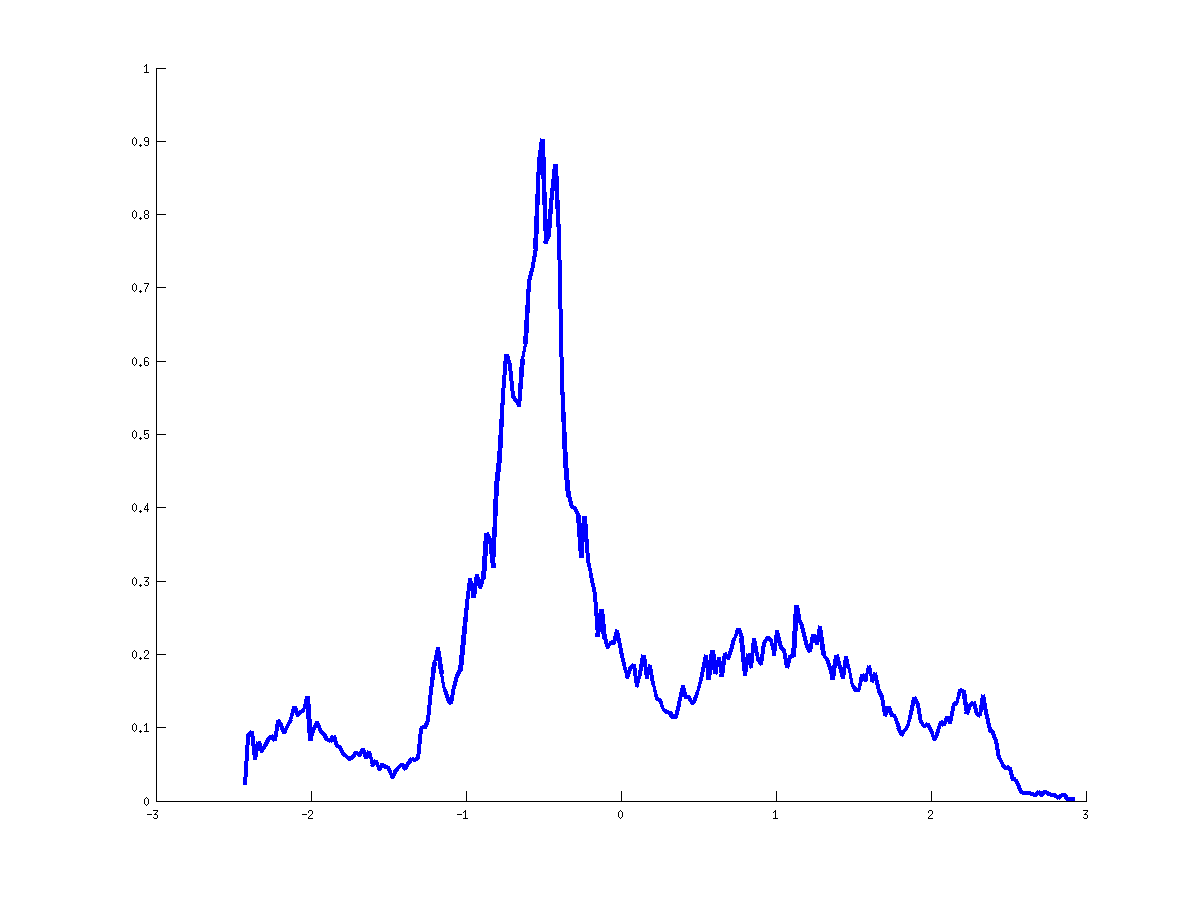
\includegraphics[width=\linewidth]{h_1}
    \end{minipage}
    \begin{minipage}{0.3\linewidth}
    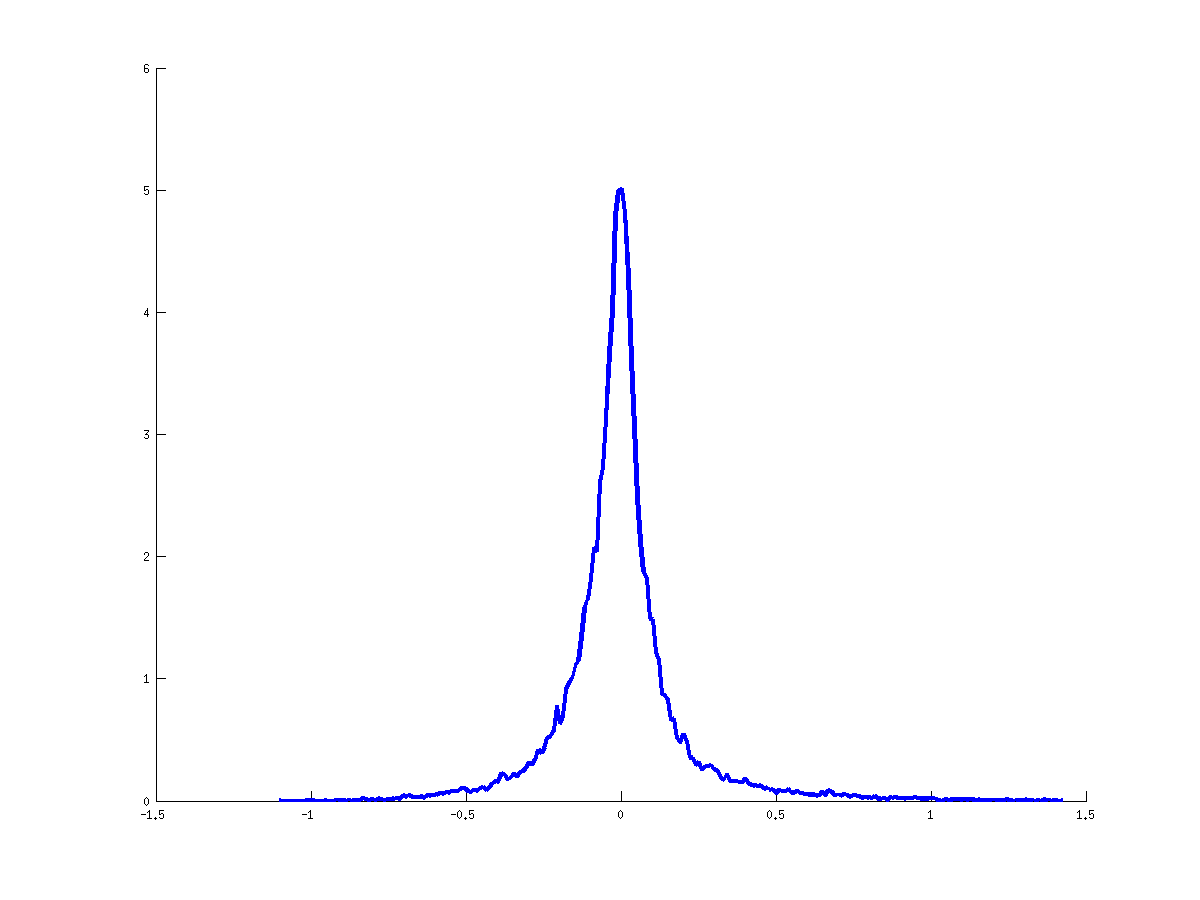
\includegraphics[width=\linewidth]{h_2}
    \end{minipage}
    \begin{minipage}{0.3\linewidth}
    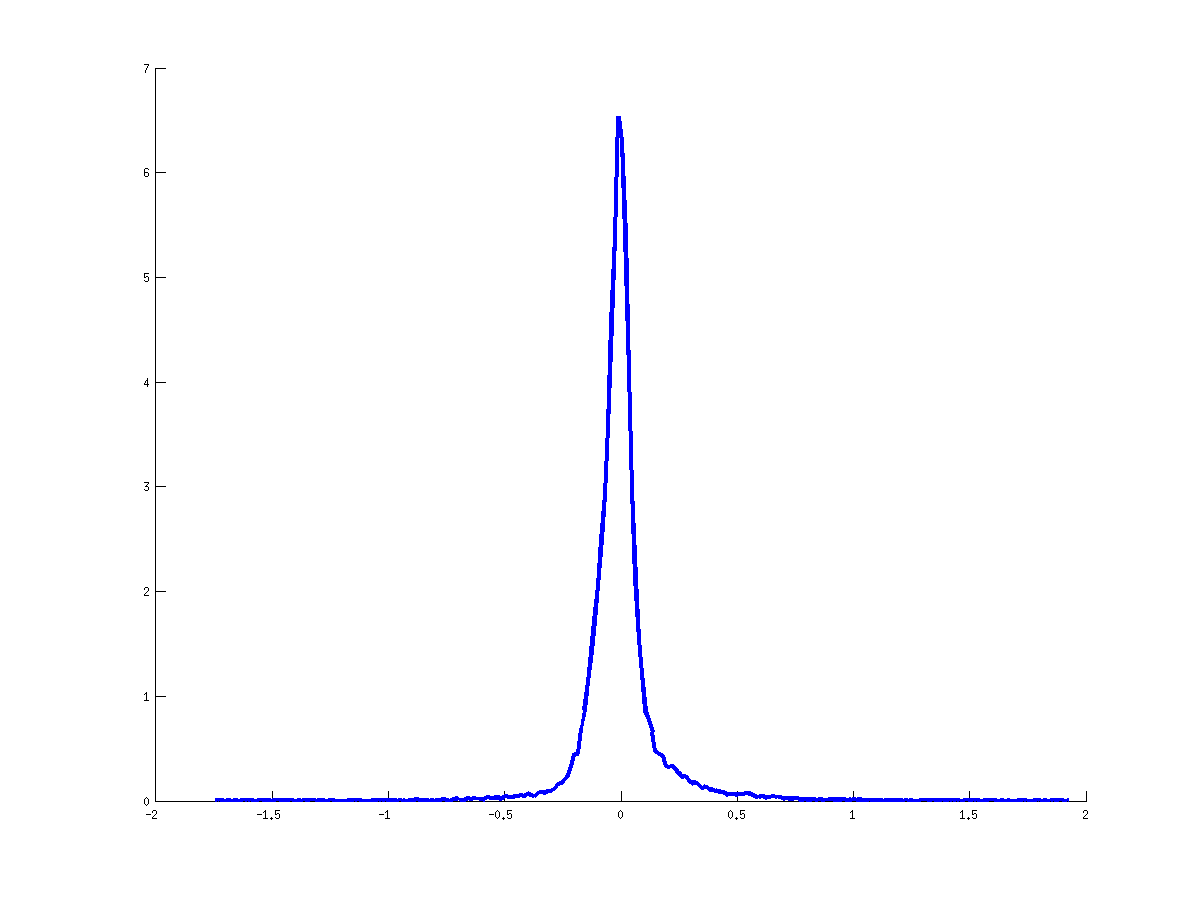
\includegraphics[width=\linewidth]{h_3}
    \end{minipage}
    \begin{minipage}{0.3\linewidth}
    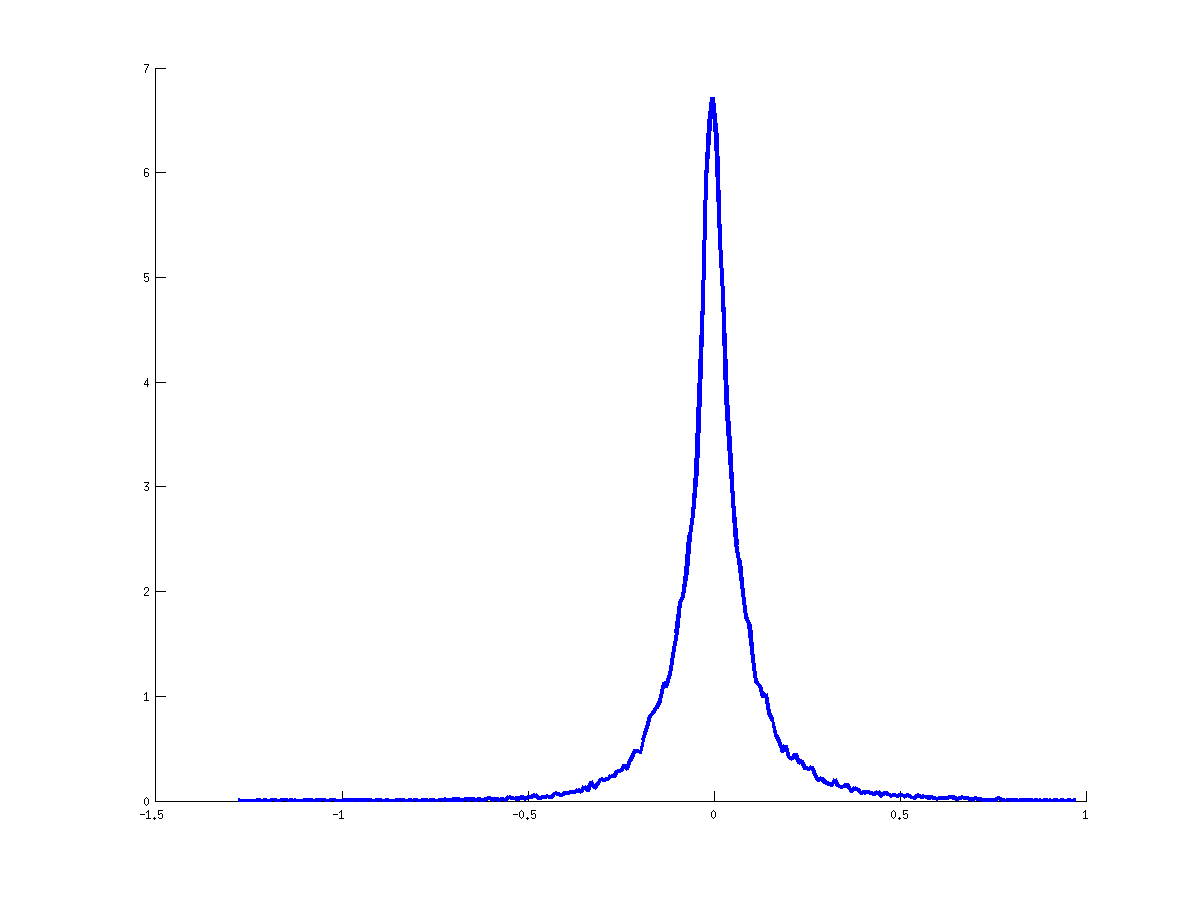
\includegraphics[width=\linewidth]{h_4}
    \end{minipage}
    \begin{minipage}{0.3\linewidth}
    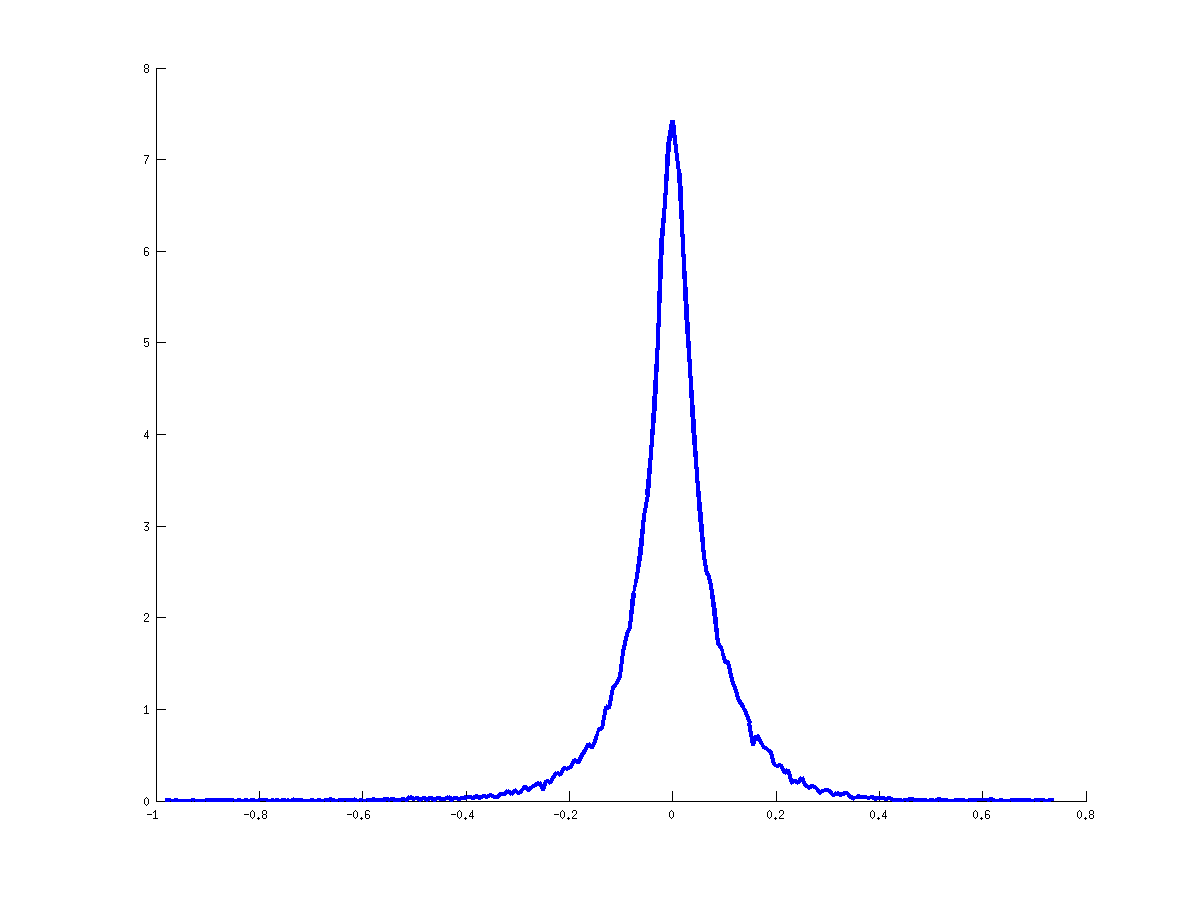
\includegraphics[width=\linewidth]{h_5}
    \end{minipage}
    \begin{minipage}{0.3\linewidth}
    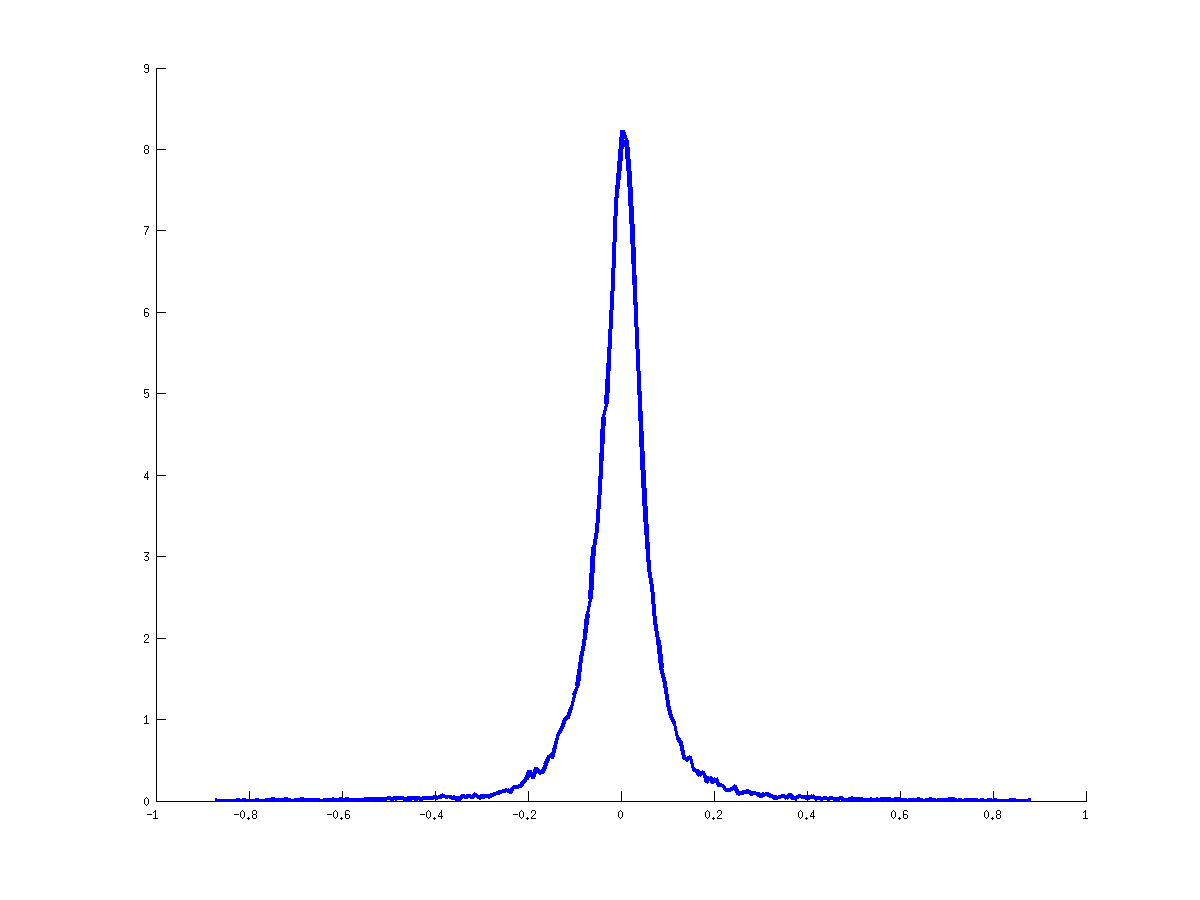
\includegraphics[width=\linewidth]{h_6}
    \end{minipage}
      \caption{The empirical histogram of the first principle component patches;}
      \label{hist}
  \end{figure}  
More precisely, Fig. \ref{para} proves that the laplace distributions fit these histograms very well. To summarizer, it is how we are simulating a image patch:
\begin{itemize}
 \item A PCA is performed to define the reference patches. (We can replace this step by a DCT).
 \item Margin distributions are modeled by laplace distribution, or gaussian distribution. Parameters are learned using their maximum likelihood estimators.
 \item Patches are simulated as $\rand{B}=\sum_i \rand{C}_i \mat{B}_i$ where $\rand{C}_i$ follows the margin distribution learned above.
\end{itemize}

\insertTwoF{h_2_gau}{h_4_gau}{In blue, the histograms of margin distributions; in red, the closest gaussian distribution in the sense of maximum likelihood; in green, the closest laplace distribution.}{0.45}{para}

\section{Likelihood Ratio with A Contrario Prior}
In this section, we combine the likelihood ration and the \textit{a contrario} prior model to build a statistic similarity criterion for patch comparison.
\subsection{Model}
First, we consider the classic noisy patch model. Let $\thetab$ be a noise free patch, distributed according to the \textit{a contrario} model. The observed patch $\xb$ is modeled by $\xb=\thetab + \nb$, where $\nb$ is a isotropic gaussian white noise, with $\sigma$ as standard deviation.  
Let's recall the likelihood ratio expression:
\begin{equation}
 \mathcal{L}(\mathbf{x}_1,\mathbf{x}_2)=
\frac{\int_{\mathbf{t \in \mathcal{R}^p}} p(\mathbf{x}_1|\boldsymbol{\theta}_{12}=\mathbf{t}) p(\mathbf{x}_2|\boldsymbol{\theta}_{12}=\mathbf{t})p(\boldsymbol{\theta}_{12}=\mathbf{t})\mathrm{d}\mathbf{t}}{\prod_{j=1,2}\int_{\mathbf{t \in \mathcal{R}^p}} p(\mathbf{x}_j|\boldsymbol{\theta}_{j}=\mathbf{t}) p(\boldsymbol{\theta}_{j}=\mathbf{t})\mathrm{d}\mathbf{t}}
\label{like}
\end{equation}
Gaussian white noise implies that 
\[
p(\xb|\thetab)\propto\exp\left(\frac{|\mathbf{x}-\boldsymbol\theta|^2}{2\sigma^2}\right)
\]
As the gaussian noise is isotropic and the basis $(\mat{B}_i)_i$ is orthogonal, we can separate the $\exp$. Let's denote $\xb=\sum_i x_i \mat{B}_i$ and $\thetab=\sum_i c_i \mat{B}_i$
\[
p(\xb|\thetab)\propto \prod_i \exp(-\frac{(x_i-c_i )^2}{2\sigma^2})
\]
The \textit{a contrario} model gives,
\[
\begin{split}
p(\thetab=\mathbf{t})\dt &=p(\thetab=\sum_i c_i \mat{B}_i) \prod \mathrm{d} c_i\\
&=\prod_i H_i(c_i) \mathrm{d} c_i
\end{split}
\]
Thus, Equ. \ref{like} can be computed along each dimension, namely:
\begin{equation}
 \mathcal{L}(\mathbf{x}_1,\mathbf{x}_2)=\prod_i \frac{\int_{c_i\in \mathcal{R}} \exp(-\frac{1}{2\sigma^2}(x_{i,1}-c_i )^2 -\frac{1}{2\sigma^2}(x_{i,2}-c_i )^2) H_i(c_i) \mathrm{d} c_i }
 {\prod_{j=1,2}\int_{c_i\in \mathcal{R}} \exp(-\frac{1}{2\sigma^2}(x_{i,j}-c_i )^2) H_i(c_i) \mathrm{d} c_i }
\end{equation}
The integral can be computed analytically if we approximate $H_i$ by gaussian distributions (not for laplace). In general, this ratio 
need to be computed using a differential schema for the integral, which is computationally expensive. In order to understand this approach, we focus on the a posteriori probability (MAP) ratio.
\begin{equation}
 \mathcal{P}_G (\mathbf{x}_1,\mathbf{x}_2)=\prod_i \frac{\sup_{c_i\in \mathcal{R}} \exp(-\frac{1}{2\sigma^2}(x_{i,1}-c_i )^2 -\frac{1}{2\sigma^2}(x_{i,2}-c_i )^2) H_i(c_i)  }
 {\prod_{j=1,2}\sup_{c_{i,j}\in \mathcal{R}} \exp(-\frac{1}{2\sigma^2}(x_{i,j}-c_{i,j} )^2) H_i(c_{i,j})  }
\end{equation}

\subsection{Studying}
\subsubsection{Gaussian Prior}
In this part, we will develop the calculus for $H_i$ gaussian with means $\mu_h$ and variance $\sigma_h^2$ (It is similar for the Laplace case, but a little more complicate). Without lost of generality, we only need to work on one component:
\[
 \mathcal{P}_{G_i} = \frac{\sup_{c\in \mathcal{R}} \exp(-\wdist{x_1}{c}{\sigma^2}-\wdist{x_2}{c}{\sigma^2}-\wdist{\mu_h}{c}{\sigma_h^2}) }
{\prod_{j=1,2}\sup_{c_j\in \mathcal{R}} \exp(-\frac{1}{2\sigma^2}(x_j-c_j )^2-\wdist{\mu_h}{c_j}{\sigma_h^2})  }
\]
Where, $\mathcal{P}_{G_i}$ denote the a posteriori ratio for the $i$th component. The optimal $c, c_j$ can be computed easily (quadratic form), and finally we have:
\begin{equation}
 -\log \mathcal{P}_{G_i}= C_i [ (x_{1,i}-x_{2,i})^2 -2b_i(x_{1,i}-\mu_{h_i})(x_{2,i}-\mu_{h_i})]
 \label{for1}
\end{equation}
where,
\[b_i=(\frac{\sigma}{\sigma_{h_i}})^2\text{, }C_i=\frac{1}{2\sigma^2(1+b_i)(2+b_i)}\]
\insertF{curve}{The behavior of the proposed distance (c.f. \ref{for1}) versus the euclidian distance. We fix a coefficient $x_1=0.5$ and we draw $y=dist(x_1,x_1+t)$}{0.8}{curv}. In red we have the euclidian distance, and in blue, the proposed distance under different values of parameter $b_i$.
Fig. \ref{curv} shows the behavior of the proposed distance. We can interpret the formula (\ref{for1}) as following:
\begin{itemize}
 \item The term $C_i$ gives the weighting for different component according to the noise level ($\sigma$) and the margin of the component ($\sigma_{h_i}$).
 \item The proposed distance is almost a euclidian distance, penalized by the deviation of the coefficient $x_1$, $x_2$ from the mean value $\mu$. More precisely, if both $x_1>\mu$ and $x_2>\mu$ (\textit{resp.} $x_i<\mu$) the distance is reduced, and the more $x_1$ and $x_2$ are far from $\mu$, the closer they are. It means the proposed distance favor rare patches for similarity.
 \item On the other hand, if $x_1-\mu$ and $x_2-\mu$ are different sign, a penalization is add to the euclidian distance. 
\end{itemize}
This gives us a rough idea of the behavior of our criterion respected to the euclidian distance. It would have been more interesting to study the laplacian prior of the background model, in which case we are conducted to study $\inf_c (x-c)^2+b|\mu-c|$, which has a similar behavior to a soft thresholding (to be continued). 
<<<<<<< HEAD
\subsubsection{Laplace Prior}
In this part we assume that $H_i$ follows a Laplace distribution, namely:
\begin{equation}
 H_i(c) \sim \exp(-\frac{1}{b}|\mu-c|)
\end{equation}
Here, $\mu$ is the location parameter, and $b$ the scale parameter. The likelihood ratio now becomes,
\[
 \mathcal{P}_{G_i} = \frac{\sup_{c\in \mathcal{R}} \exp(-\wdist{x_1}{c}{\sigma^2}-\wdist{x_2}{c}{\sigma^2}-\frac{1}{b}|\mu_h-c|) }
{\prod_{j=1,2}\sup_{c_j\in \mathcal{R}} \exp(-\frac{1}{2\sigma^2}(x_j-c_j )^2-\frac{1}{b}|\mu_h-c_j|)  }
\]
We can now see the link between the sparsity and the Laplace distribution. More precisely, the maximum a posteriori correspond to a soft threshold. Let's introduce the proximity function (the infimum)
\[
858
\]
=======

>>>>>>> 5a0d7a55716530789aebf7704aa3f7921edcafc6
In the next section, we conceive two kind of experience in order to test the performance of the proposed similarity criterion.

\section{Experiments}
In this section we aim to test the performance of the proposed similarity criterion. In a first time, we use our method to match patch in a patch dictionary, and compare its \textbf{ROC} curve (Receiver operating characteristic) to the euclidian distance. Secondly, we modify the non-local means denoising method by using our proposed criterion to check out both the PSNR and visual performance.
\subsection{ROC Curve Performance}
The ROC curve illustrates the performance of a similar criterion as its discrimination threshold is varied. For this, we match noisy patches from a fixed dictionary by using our similarity criterion, and draw the PFA-PTD curve. 
\begin{itemize}
 \item PFA, probability of false alarm, is the probability to decide $\mathcal{H}_1$ under $\mathcal{H}_0$.
 \item PTD, probability of true detection, is the probability to decide $\mathcal{H}_1$ under $\mathcal{H}_1$.
\end{itemize}

We use the same patch dictionary as Deledalle \textit{et al.}\cite{Deledalle:2012} (Fig. \ref{dico}). The experience consists in matching two noisy versions of this dictionary and evaluate the similarity criterion used for the matching. Typically we are going to compare the performance of our method with the euclidian distance. 
\insertTwoF{dico}{dico_noise}{Left, the patch dictionary proposed by Deledalle \textit{et al.}\cite{Deledalle:2012}; right, the noisy version that we used for matching}{0.45}{dico}
The proposed method need a prior learning step and one parameter $\sigma$ for the likelihood term, so we are going to show the performance under the change of these conditions.
  \begin{figure}[!h]
    \centering
    \begin{minipage}{0.45\linewidth}
    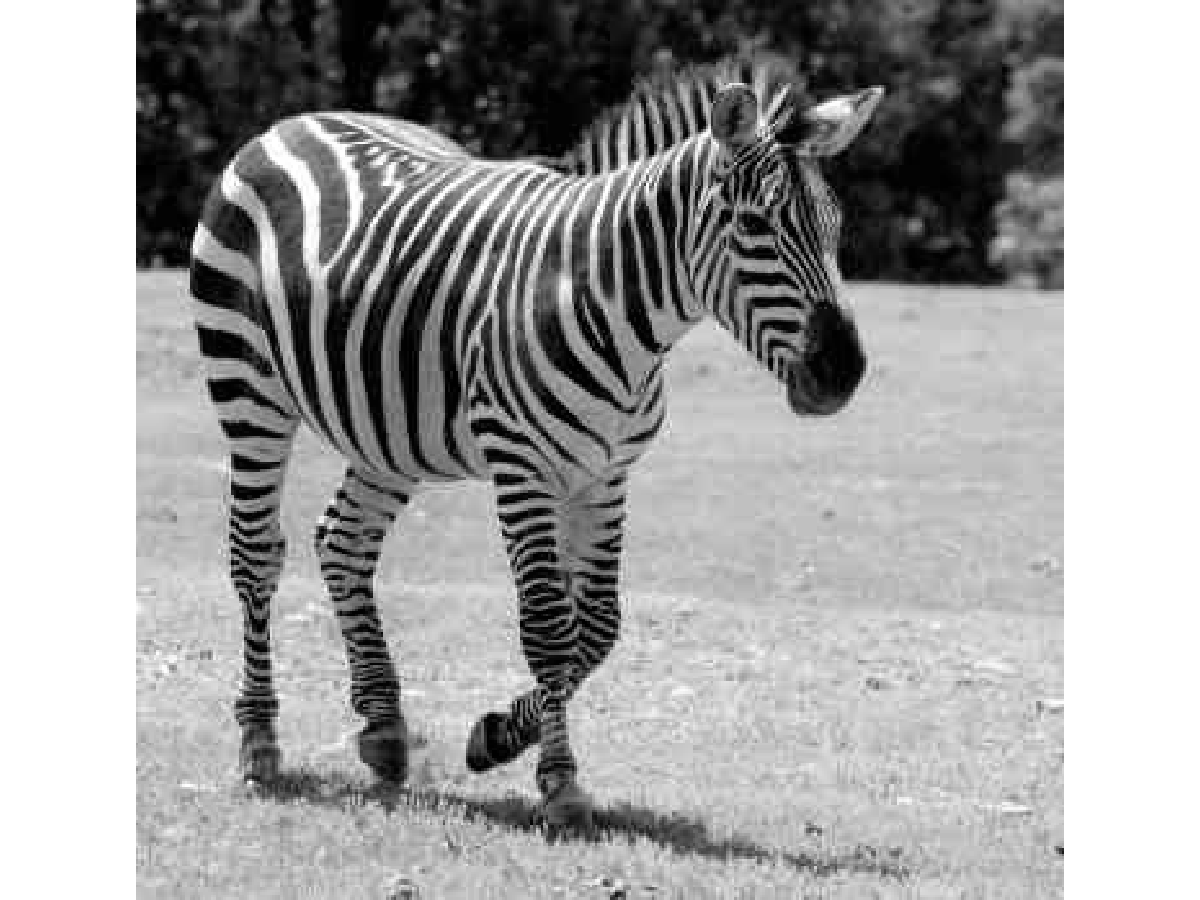
\includegraphics[width=\linewidth]{zebra}
    \end{minipage}
    \begin{minipage}{0.45\linewidth}
    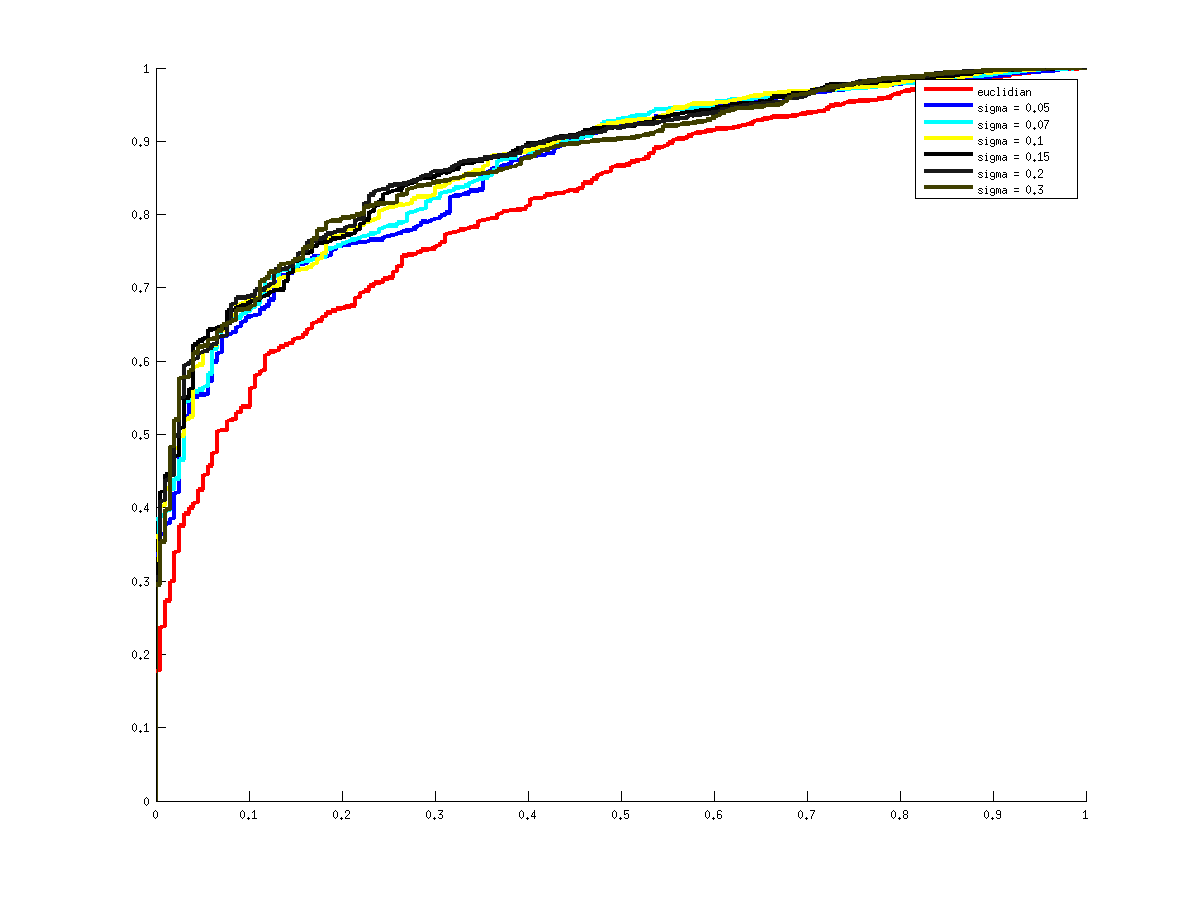
\includegraphics[width=\linewidth]{perf_zebra_max}
    \end{minipage}
    \begin{minipage}{0.45\linewidth}
    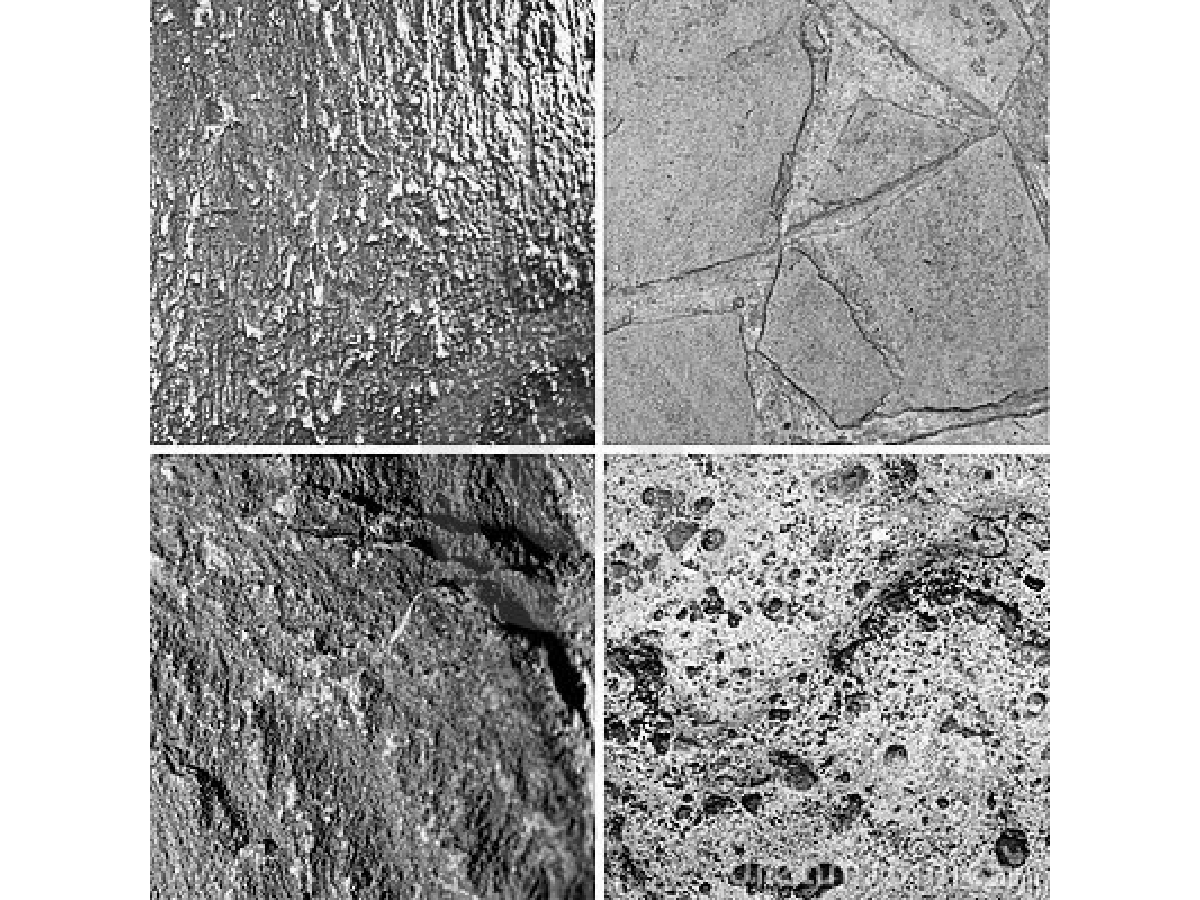
\includegraphics[width=\linewidth]{texture}
    \end{minipage}
    \begin{minipage}{0.45\linewidth}
    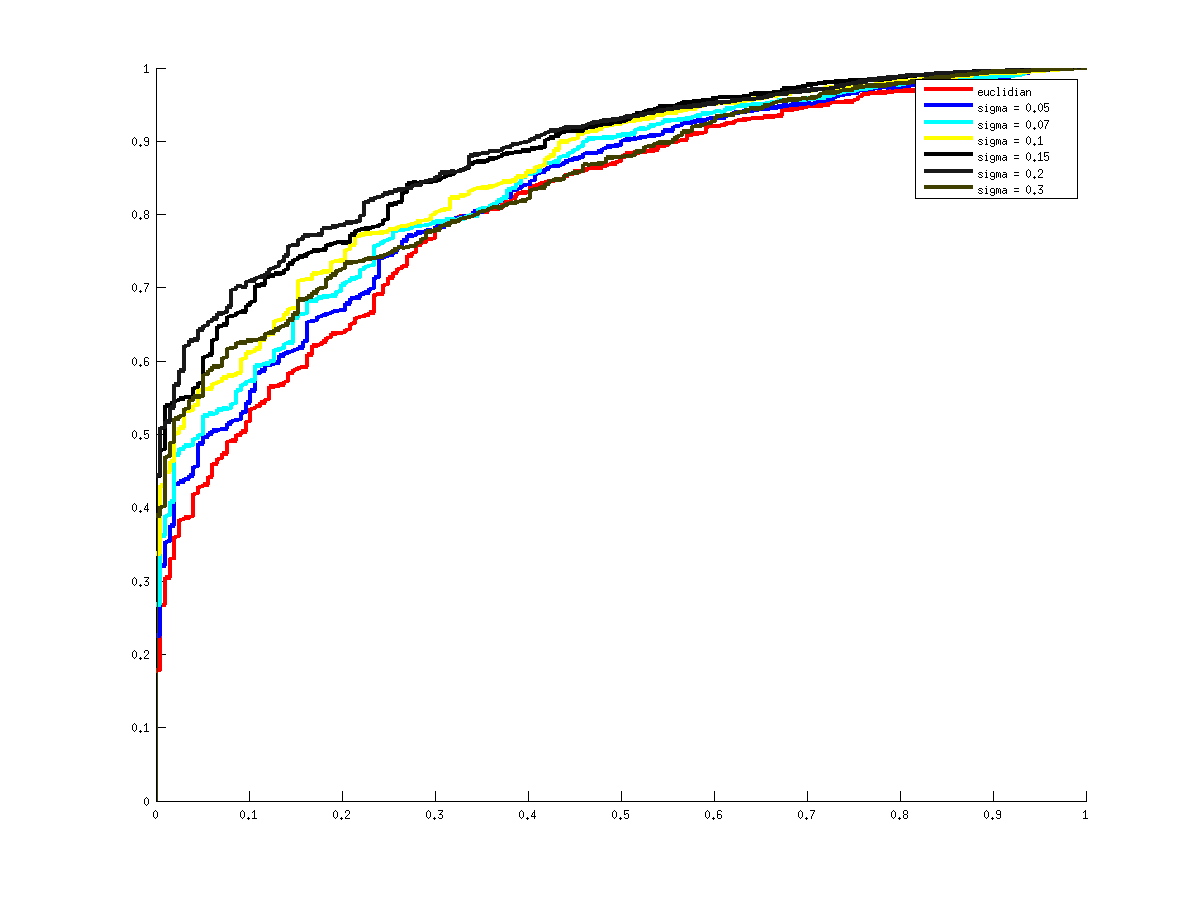
\includegraphics[width=\linewidth]{perf_texture_max}
    \end{minipage}
      \caption{Left: the image used for prior learning; right:  the ROC performance of our method (in multi colors for different $\sigma$) versus the euclidian distance (in red)}
      \label{perf}
  \end{figure}  
Fig.\ref{perf} illustrates the performance of our method versus the euclidian distance. First of all, our method is significant better than the euclidian distance. Secondly, a noise of 75 standard deviation is added, and the best performance is obtained by setting $\sigma=32$ in the proposed method. And we observe under different $\sigma$ the best performance is always obtained by setting $\hat \sigma=\frac{1}{2} \sigma$, where $\hat \sigma$ is the parameter in our model and $\sigma$ is the real noise deviation. 
Finally, as we expected, if the prior is learned from a gaussian white noise image, we get the same performance as the euclidian distance. (Fig. \ref{wn})
\insertTwoF{wn}{perf_wn_max}{The performance of the proposed method using a white noise prior.}{0.45}{wn}
\subsection{Statistic Similarity for Non Local Means Denoising}
We implement the classic non local means denoising method \cite{Buades:2005} by changing the weighting function. Given a reference patch $\mat{B}_r$, \cite{Buades:2005} propose to weight the patches in a sub window centered on $\mat{B}_r$ according to their euclidian distance $D_j=\lVert \mat{B}_r- \mat{B}_j \rVert^2$. The non-local mean filter compute a denoised patch $\tilde{\mat{B}}_r$ as
\begin{equation}
 \tilde{\mat{B}}_r=\sum_j K_j \mat{B}_j
\end{equation}
where the weights $K$ are computed as
\[
K_j=\frac{\tilde{K_j}}{\sum_j \tilde{K_j}}\text{, and  } \tilde{K_j}=\exp(-\frac{1}{2\tau^2} D_j)
\]
where $\tau$ is a parameter of the model.

To illustrate the performance of the proposed criterion, we only need to switch the euclidian distance to the $-\log \mathcal{P}_{G}$, by defining:
\[
\tilde{D}_j=-\log \mathcal{P}_{G}(\mat{B}_r,\mat{B}_j)
\]

  \begin{figure}[!h]
    \centering
    \begin{minipage}{0.45\linewidth}
    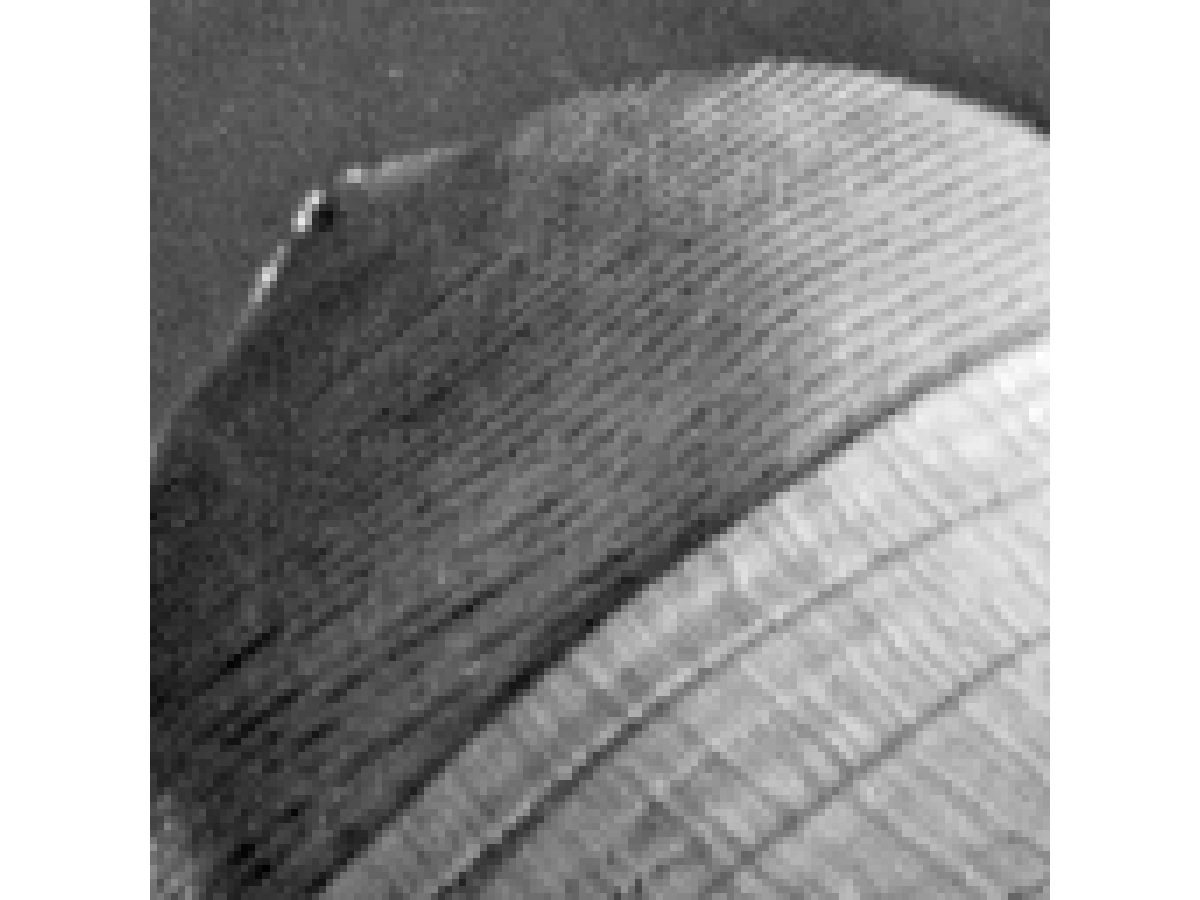
\includegraphics[width=\linewidth]{hat_origine}
    \end{minipage}
    \begin{minipage}{0.45\linewidth}
    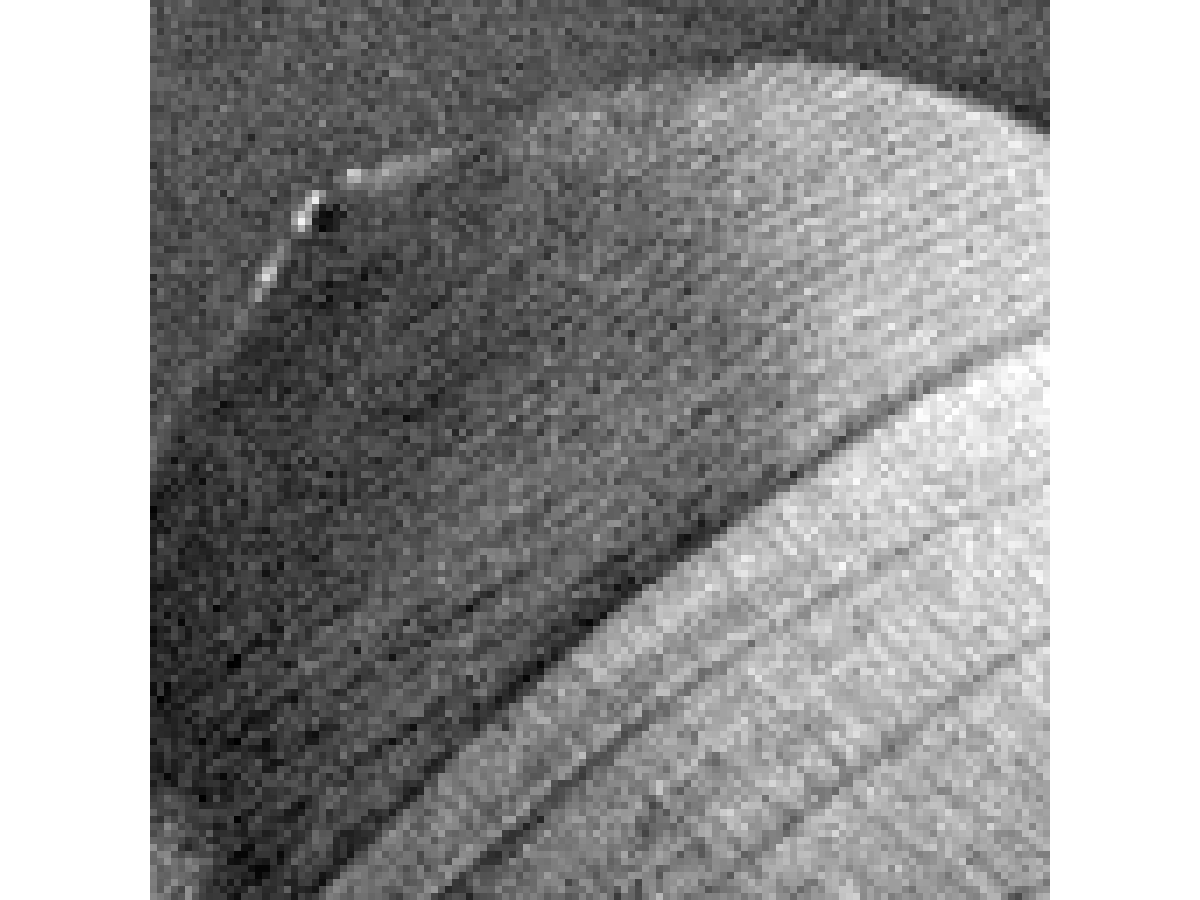
\includegraphics[width=\linewidth]{hat_noisy}
    \end{minipage}
    \begin{minipage}{0.45\linewidth}
    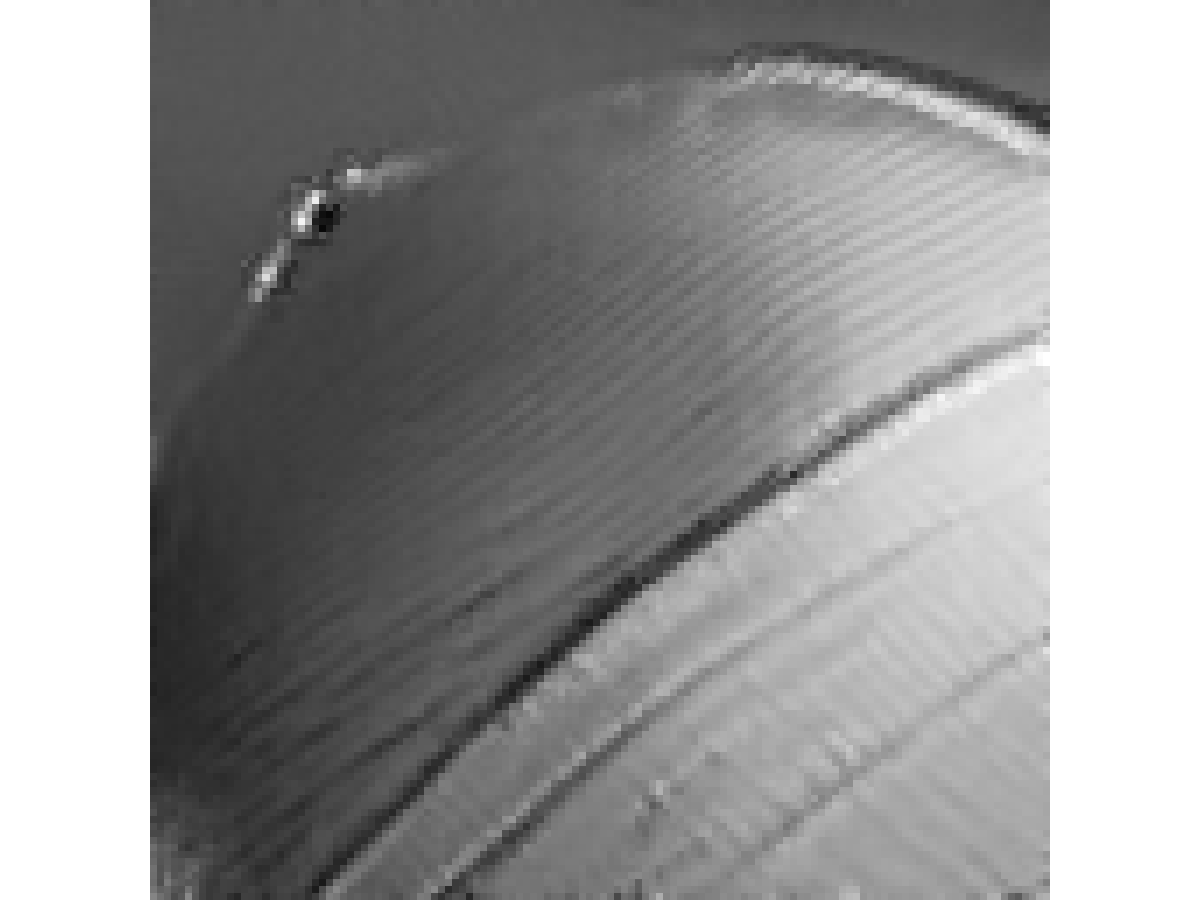
\includegraphics[width=\linewidth]{hat_eucli}
    \end{minipage}
    \begin{minipage}{0.45\linewidth}
    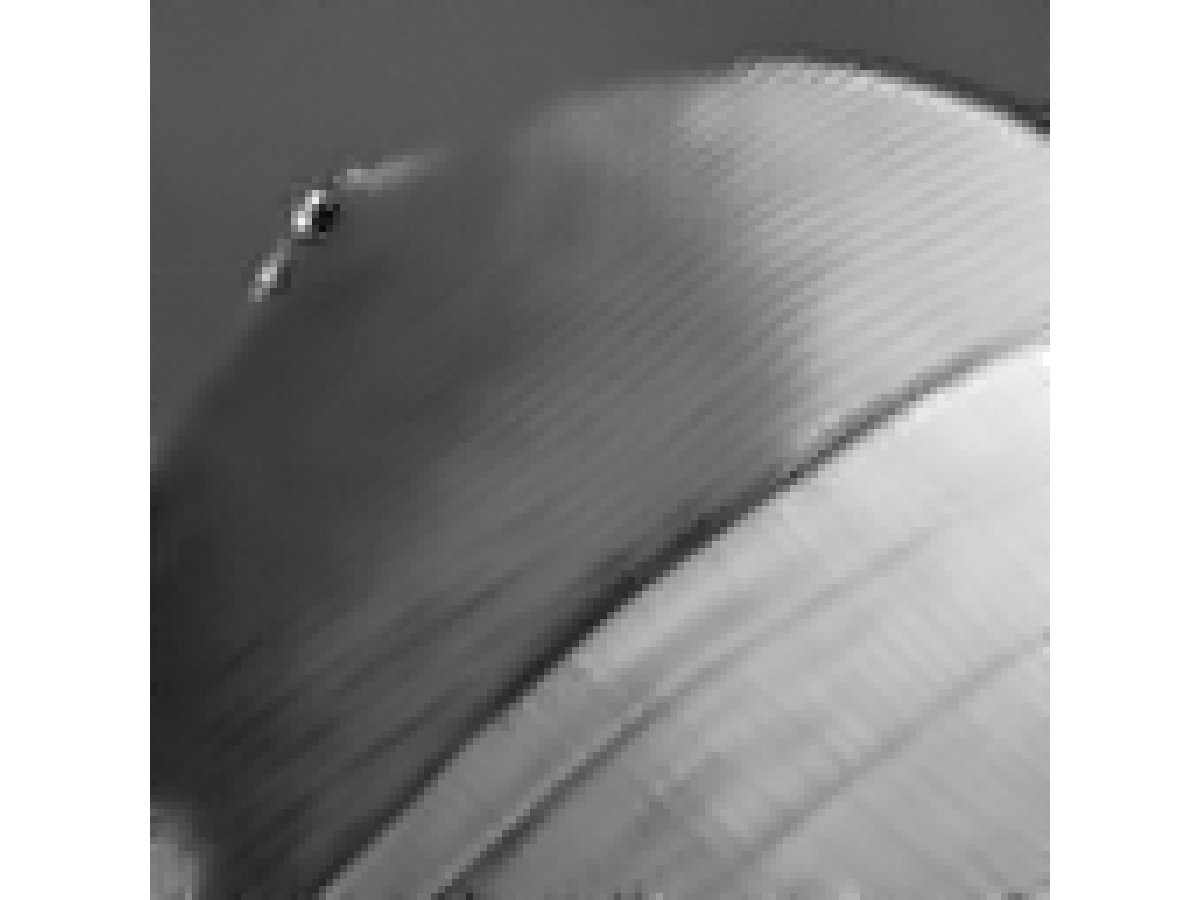
\includegraphics[width=\linewidth]{hat_our}
    \end{minipage}
      \caption{Top right: the origin image; Top left: noisy image with $\sigma=15$; Bottom left: denoising with classic NL means,$PSNR=20.5$; Bottom right: denoising with our NL means, $PSNR=22.8$;}
      \label{lena_de}
  \end{figure}  
  
  \begin{figure}[!h]
    \centering
    \begin{minipage}{0.45\linewidth}
    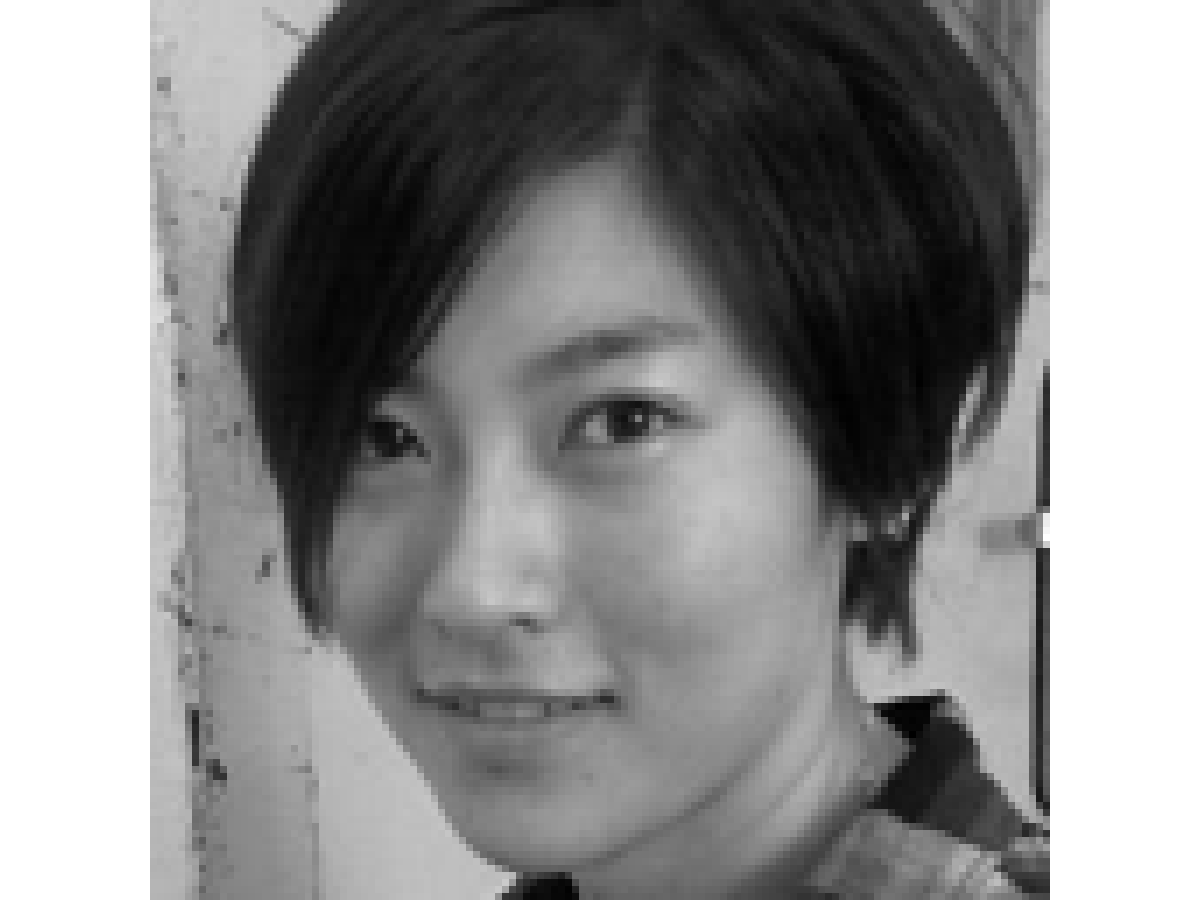
\includegraphics[width=\linewidth]{byzh_origine}
    \end{minipage}
    \begin{minipage}{0.45\linewidth}
    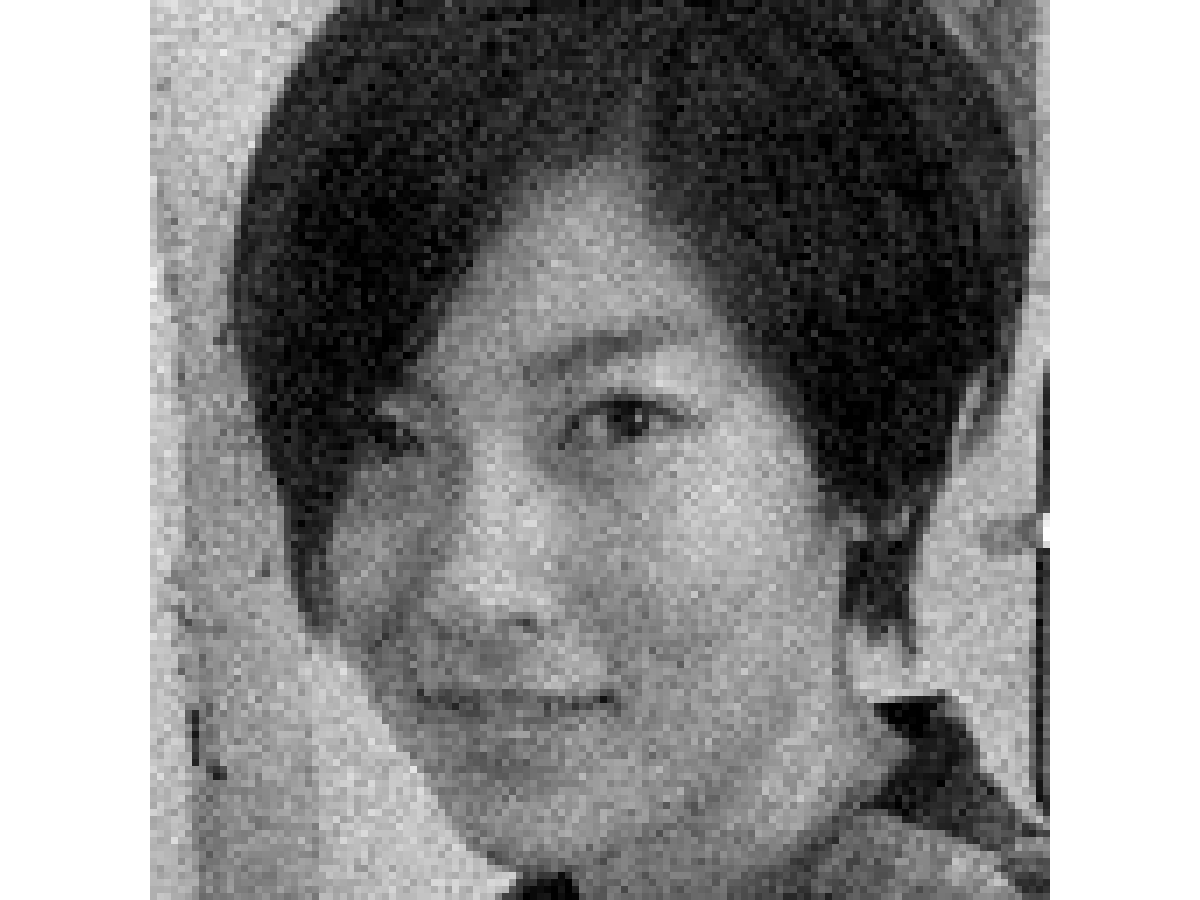
\includegraphics[width=\linewidth]{byzh_noisy}
    \end{minipage}
    \begin{minipage}{0.45\linewidth}
    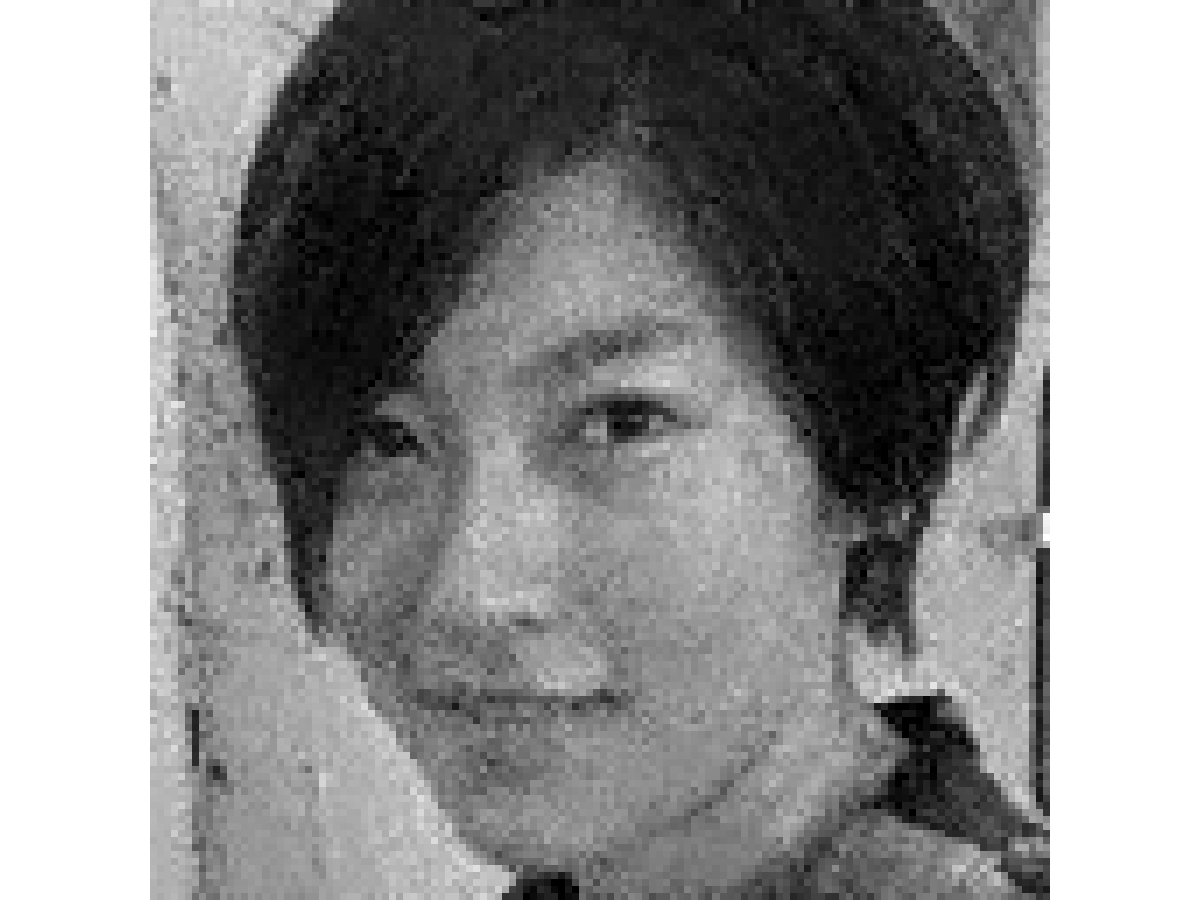
\includegraphics[width=\linewidth]{byzh_eucli}
    \end{minipage}
    \begin{minipage}{0.45\linewidth}
    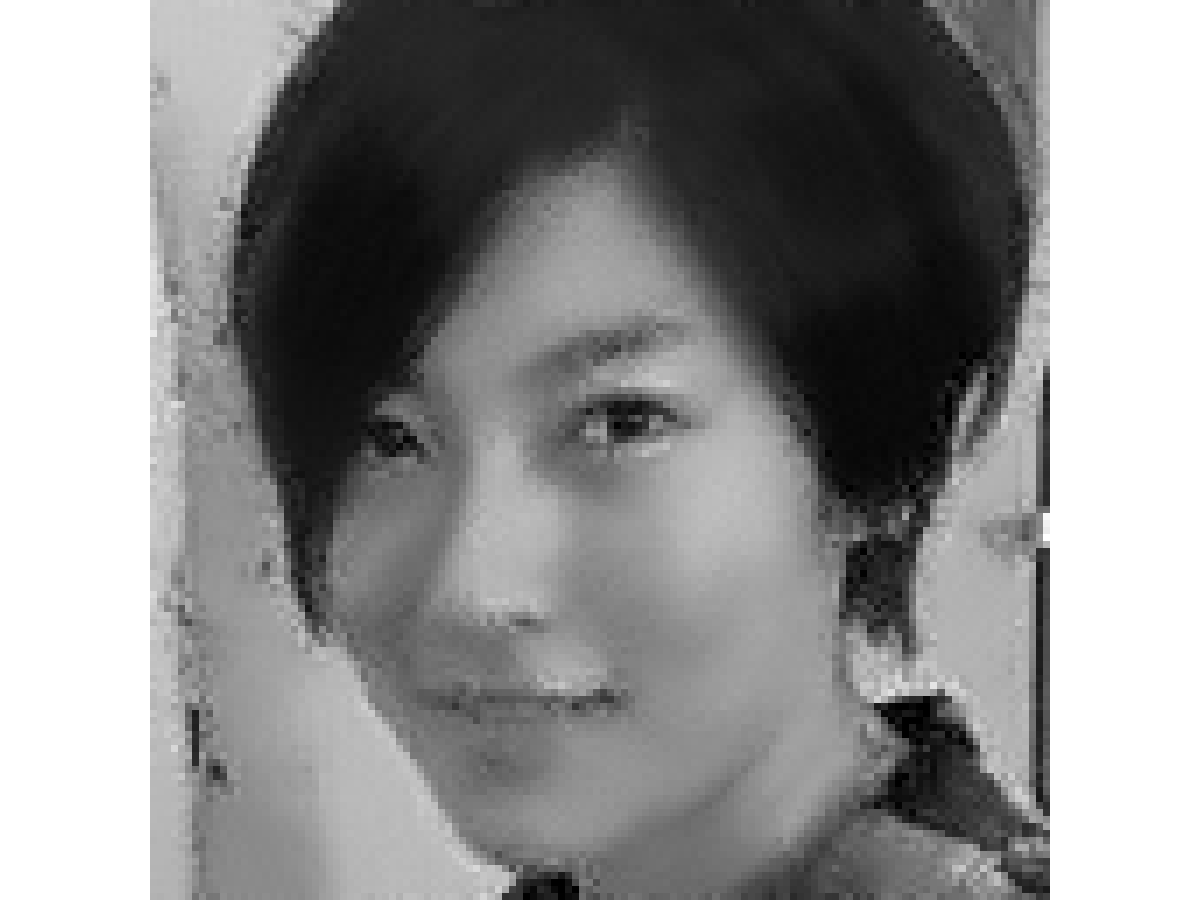
\includegraphics[width=\linewidth]{byzh_our}
    \end{minipage}
      \caption{Top right: the origin image; Top left: noisy image with $\sigma=15$; Bottom left: denoising with classic NL means,$PSNR=20.6$; Bottom right: denoising with our NL means, $PSNR=24.5$;}
      \label{byzh_de}
  \end{figure}  
\section{Conclusion}

In this project, we have combined the \textit{a contrario} model and the likelihood ratio to give a new statistic patch comparison criterion. We evaluate its performance by drawing its ROC curve and inserting it into a classic NL means denoising algorithm. We see that in both case, we beat the euclidian distance. For the futur, the next things should be done:
\begin{enumerate}
 \item Studying the case of laplacian prior and evaluating the performance.
 \item Finding out how to fix automatically the parameters.
 \item Comparing to more sophisticates patch similarity criterion, such as the one proposed by \cite{Dabov:2006}, used in the BM3D algorithm (a hard thresholding distance in a linear transformed domain, DFT, DCT), trying to generalizing the our method. 
\end{enumerate}

\newpage

\bibliographystyle{splncs}
\bibliography{patch}
\end{document}
